%HEADER
%%%%%%%%%%%%%%%%%%%%%%%%%%%%%%%%%%%%%%%%%%%%%%%%%%%%%%%%%%%%
\documentclass[a4paper, %Format
		11pt, %Font size
		headsepline,
%toc - table of content
		toc=listof, %Include TOC
		toc=listofnumbered, %Number TOC
		toc=bibliography, %Literaturverzeichnis ins TOC
		toc=bibliographynumbered, %Literaturverzeichnis im TOC nummerieren
		]{scrreprt} %Doc class[Optionen]

%Bibliography
%\usepackage{cite} %Paket für Literaturverweise
\usepackage[backend=biber, sorting=none]{biblatex}
\addbibresource{literatur.bib}
%\bibliography{literatur.bib} %Literaturverzeichnis

%GEOMETRIE UND AUSSEHEN
\usepackage[left=35mm,right=30mm,top=15mm,bottom=25mm]{geometry} %Set text geometry
\linespread{1.3}
\setlength{\parindent}{0pt} %disable first line spacing
\usepackage{microtype} %automatically adjust distance between letters

\usepackage{color} %Colorpackage
\definecolor{lightgrey}{rgb}{0.97,0.97,0.97} %definition von "lightgrey"
\usepackage[skip=2pt,font=footnotesize]{caption}


%SONDERZEICHEN UND DEUTSCHE ÜBERSETZUNG
%\usepackage{ucs}<
\usepackage[utf8]{inputenc} %UTF-8 
\usepackage[ngerman, english]{babel}
\usepackage{csquotes}
\usepackage[text]{}
\usepackage{gensymb}

%Tables
\usepackage{booktabs} %extended table options
\usepackage{multirow} %table elements over multiple rows
\usepackage{csvsimple}

%Graphs
\usepackage{graphicx} %Insert graphics
\usepackage{subfig}
\usepackage{xcolor}
\definecolor{titlepagecolor}{cmyk}{1,.60,0,.40}
\definecolor{namecolor}{cmyk}{1,.50,0,.10} 

%Sourcecode
\usepackage{scrhack}
\usepackage{listings} %u.a. Darstellen von Sourcecode
\renewcommand\lstlistingname{Quelltext} %Übersetzung/Umbenennung von "listing" in "Quelltext"
\renewcommand\lstlistlistingname{Quelltextverzeichnis} %Übersetzung von "Quelltextverzeichnis"
%Darstellungsoptionen von Sourcecode
\lstset{numbers=left, numberstyle=\tiny, stepnumber=1, captionpos=b, backgroundcolor=\color{lightgrey}, breaklines=true; float=htbp;} 

%TOC
\usepackage{titletoc}
%\dottedcontents{chapter}[1.5em]{ }{2.3em}{1pc}

%Footnotes
\usepackage{chngcntr}
\counterwithout{footnote}{chapter} %durchgehende, kapitalübergreifende Nummerierung
\setlength{\skip\footins}{10mm} % bestimmt den Abstand zwischen der Grenzlinie der Fußnoten und dem Fließtext.


%Head and Bottom line
\usepackage[singlespacing=true]{scrlayer-scrpage} %Paket für Kopf/Flusszeilen
%\renewcommand*{\chapterpagestyle}{scrheadings} %Seite eines Kapitelbeginn: Linie in Kopfzeile,

%HYPERLINKS
\usepackage{url} %Erleichtert Darstellung von URL (viele Sonderzeichen)
\usepackage[pdftex]{hyperref} %Erstellt Hyperlinks im PDF
% Nach "hyperref" sollten keine weiteren Pakete eingebunden werden,
% da "hyperref" gewisse Befehle umdefiniert.

%%%%%%%%%%%%%%%%%%%%%%%%%%%%%%%%%%%%%%%%%%%%%%%%%%%%%%%%%%%%
%DOKUMENT
\begin{document}

% \clearpairofpagestyles %löscht bisherige Kopf-Fusszeilen Definitionen
% \headsepline{0pt} %Definition der Linienstärke in der Kopfzeile, hier 0

\startcontents[main] % Start TOC

\thispagestyle{empty}
\begin{titlepage}
%\center
\includegraphics[width=140mm]{Pictures/TitlepageHead}
\newgeometry{left=5.5cm} %defines the geometry for the titlepage
\pagecolor{titlepagecolor}
\noindent

\includegraphics[width=10cm]{Pictures/logo.jpg}\\[-1em]
\color{white}
\makebox[0pt][l]{\rule{1.3\textwidth}{1pt}}
\par
\noindent
\textbf{\textsf{University of Aalen}}\\
%\vfill
\noindent

\vspace{2cm}
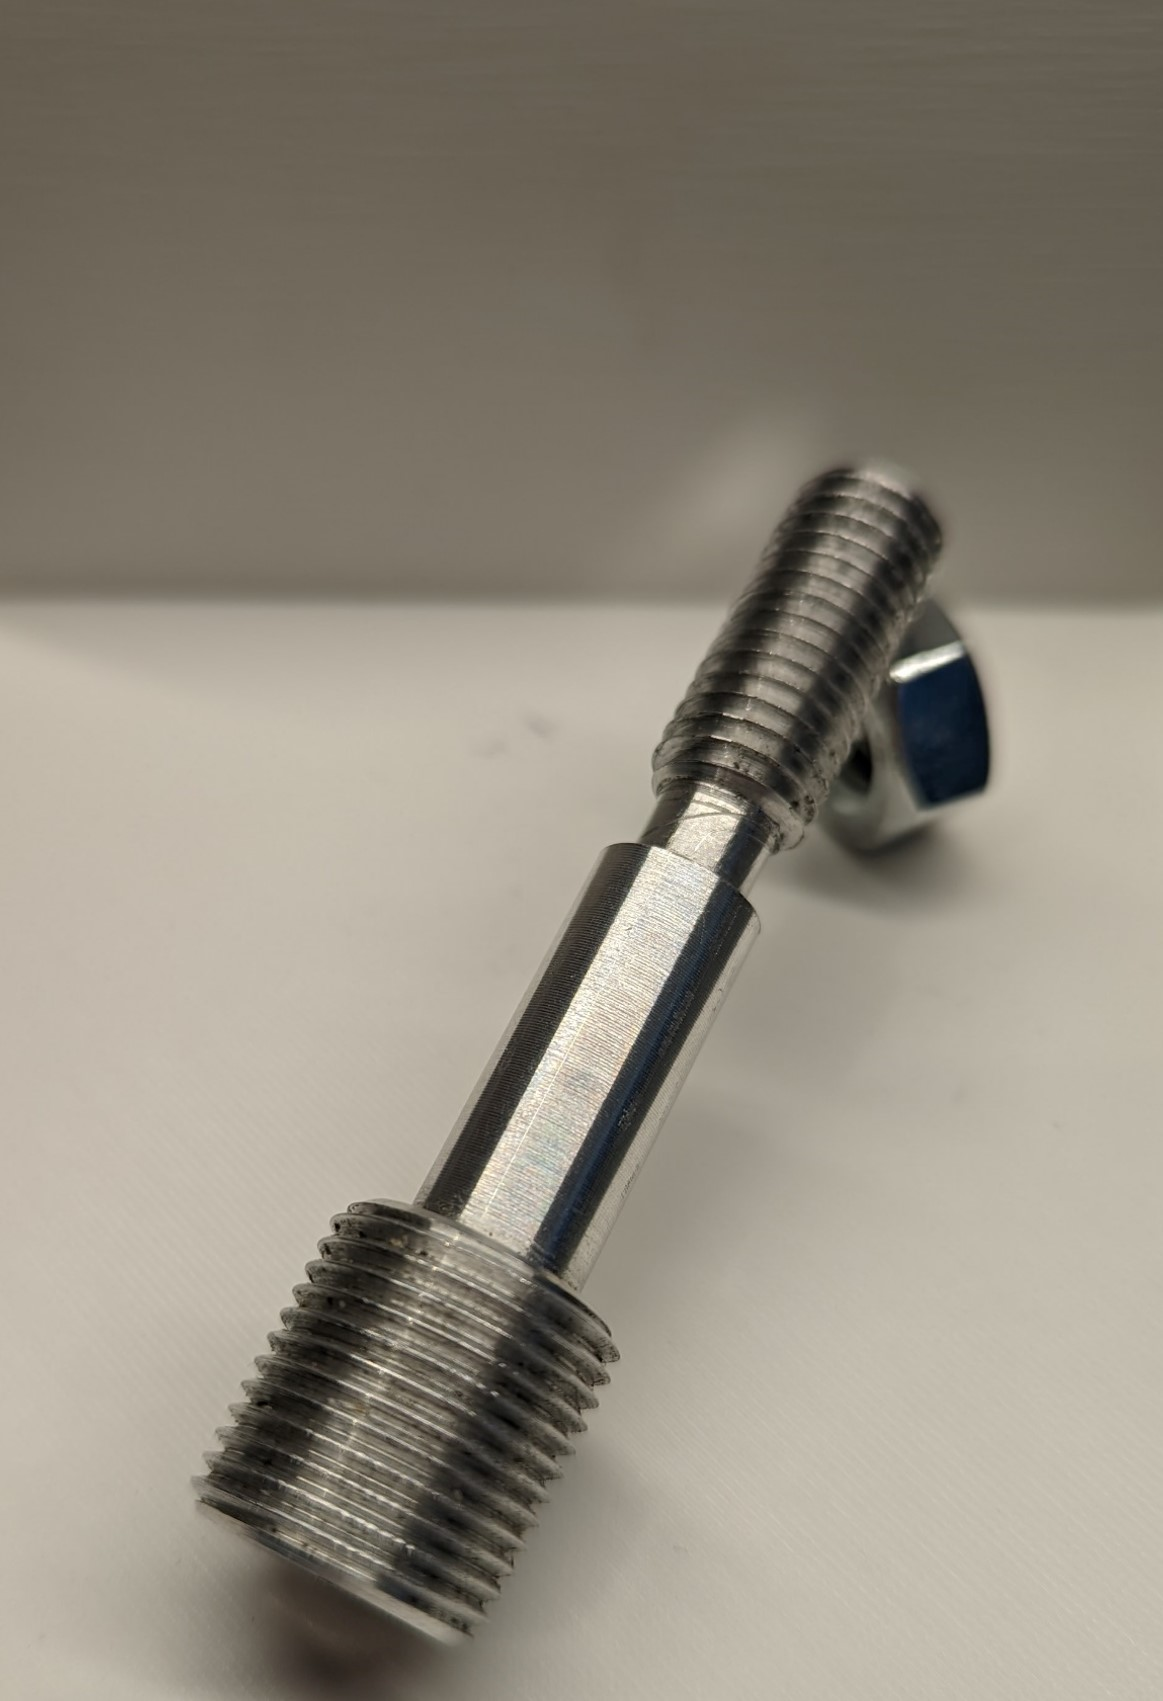
\includegraphics[width=8cm]{Pictures/Title.jpg}
\vspace{2cm}

{\huge \textsf{Mechatronic Project - Electronic Lead Screw}}
\vskip\baselineskip
\noindent
\textsf{February 2022 - Lukas Schwörer}
\end{titlepage}
\restoregeometry % restores the geometry
\nopagecolor% Use this to restore the color pages to white

%%Leerseite
\thispagestyle{empty}
\hspace{1mm}\\
\newpage

\pagenumbering{roman} %römische Seitenzahlen
\setcounter{page}{1} %Seitenzähler zurücksetzen

\thispagestyle{empty}
\chapter*{Preface}
\addcontentsline{toc}{chapter}{Preface}
\label{preface}

This project is part of the master’s degree program "System engineering" of Aalen University and is scheduled to be performed during the first two semesters of the program. This report covers the work realized from April 2021 to February 2022.\\
The practical work and the writing for this project was performed from home due to the Covid-19 Pandemic.

\vspace*{25mm}

\begin{otherlanguage}{ngerman}
    Dieses Projekt ist Teil des Masterstudiengangs ''System Engineering'' der Hochschule Aalen und muss während der ersten beiden Semester absolviert werden. Die in diesem Bericht beschriebene praktische Arbeit wurde von April 2021 bis zum Februar 2022 realisiert.\\
    Die praktische Arbeit, wie auch das Schreiben des Berichts wurde Zuhause ausgeführt aufgrund der Covid-19 Pandemie.
\end{otherlanguage} 

\thispagestyle{empty}
\chapter*{Abstract}
\addcontentsline{toc}{chapter}{Abstract}
\label{abstract}

\thispagestyle{empty}
\chapter*{Kurzfassung}
\addcontentsline{toc}{chapter}{Kurzfassung}
\label{kurzfassung}
\begin{otherlanguage}{ngerman}

    Dieses Projekt beschäftigt sich mit der Entwicklung, dem Aufbau, dem Testen und Qualifizieren einer Elektronischen Leitspindel (ELS). Dieses Projekt wurde der Universität von mir vorgeschlagen, da es aufgrund der Covid-19 Pandemie nur begrenzt möglich war praktische Projekte durchzuführen. Sein Ziel ist es ein System zu entwickeln, dass das Getriebe in einer konventionellen Drehbank ersetzt und die Rotation der Leitspindel zu der Rotation der Hauptspindel synchronisiert. Die ELS muss fähig sein, mit der Rotation der Hauptspindel mitzuhalten während einer konventionellen Drehbearbeitung mit unterschiedlichen Drehzahlen und Vorschüben. Zusätzlich muss es möglich sein, präzise metrische und imperische Gewinde herzustellen.\\
 
    Das elektromechanische System der ELS besteht aus einem Encoder, der die Position der Hauptspindel ausliest und einem Servomotor, der die Position der Leitspindel kontrolliert. Ein Mikrocontroller
    verarbeitet die vom Encoder gesammelten Informationen und bestimmt die korrekte Position des Servomotors.\\
    Um ein einfaches Ändern und Entfernen von Features zu ermöglichen und das Verhalten des Systems vorherzusagen, muss die Entwicklung der ELS Modellbasiert durchgeführt werden. Dieses Modell muss alle Komponenten des reellen Systems beinhalten, eingeschlossen der Spindel, des Encoders, dem Mikrocontroller und dem Servomotor. Zum Vergleich sollte auch ein System mit einem konventionellen Getriebe modelliert werden.
    
\end{otherlanguage}


\thispagestyle{empty}
\chapter*{Acknowledgement}
\addcontentsline{toc}{chapter}{Acknowledgement}
\label{acknowledgement}
At this point I would like to thank the following people who made this project possible:

\begin{itemize}
\item \textbf{Person} Reason. 

\end{itemize}


% Insert TOC
\renewcommand\contentsname{\huge Table of Contents}% Change TOC Name and size
\printcontents[main]{ }{0}{\section*{\contentsname}}
\newpage

%KOPF-/FUSSZEILE
\pagestyle{scrheadings} 
% \clearpairofpagestyles %löscht bisherige Kopf-Fusszeilen Definitionen
% \automark[]{chapter} %[rechte Seite]{linke Seite}
% \chead[]{\headmark} %oben mitte
% \cfoot[\pagemark]{\pagemark} %Seitenzahlen auf [Seite des Kapitelbeginns]{den folgenden Seiten}
% \headsepline{0.5pt} %Definition der Linienstärke in der Kopfzeile, hier 0,5

\newpage
\pagenumbering{arabic} %arabische Seitenzahlen
\setcounter{page}{1} %Seitenzähler zurücksetzen

\chapter{Introduction}
\label{introduction}


\chapter{Theoretical Background}
\label{theoretical_background}

\section{Numerical Mathmatic}
\subsection{Fractional Mathmatic}
\subsection{Floatingpoint Mathmatic}

\section{Motors}

\section{Manufactoring}
\subsection{Additive Manufactoring}
\subsection{Subtractive Manufactoring}


\chapter{Hardware and Software}
\label{hardwareandsoftware}

In this Chapter the needed background information for the used hardware and software will be described.

\section{Hardware}
\subsection{Electro mechanical actuators}
\subsubsection{Stepper Motors}
\subsubsection{Closed Loop Servos}

\subsection{Microcontroller}
\subsubsection{TI LaunchXL F280049C}
\subsubsection{Logic Level Shifter}

\subsection{Raspberry Pi}
A Raspberry Pi is a Single board computer.
\subsubsection{Touchscreen}
Touchscreens can be either resistive or capacitive. The react to them being touched and are used to interact with electronic devices.

\section{Software}
\subsection{Matlab and Matlab-Simulink}
MATrix LABoratory (MATLAB) is an Integrated Development Environment (IDE)
and programming language. MATLAB was developed in the need of a numerical algebraic
system at the university of New Mexico. On this base, the company MathWorks (see
Appendix B) was created. Since 1984 MathWorks is further developing MATLAB and
%TODO add Appendix B (Companies)
additional software for numerical algebraic computing. To support different hardware
packages MathWorks offers so called toolboxes. These toolboxes contain functions and
scripts for communication, data acquisition, motion control etc.
MATLAB is mainly used in technical development and research.

\subsection{Code Composer Studio}
\subsubsection{C Code}
C is a programming language which is used when quick code execution and a small program size is needed.

\subsection{Python}
Python is a object oriented programming language.
\subsubsection{Kivy}
Kivy is a Python software Package for the creation of graphical user interfaces.

\subsection{Git}
Git is an software tool for source code management and versioning, as well as for parallel development. Git was developed by Linus Torvald in 2005. Git was developed in the need of source code management software for the development of the operating system Linux. [25]
Git allows development in so-called branches. These are independent copies of an already existing and probably used software. This ensures that modifications or enhancements are not affecting already used software. If a feature is finished, it can be merged back into the higher-level branch. Merging is the process of bringing two files, directories or branches together.
Different developers, working on different features of the same project is called parallel development.
Further Git is a tool for software versioning. Software versioning is a tracking of changes in a project. In case of an mistake the project can be recovered to every tracked point.
Git was very heavily used for software development after and during our testing. At some time 4 developers where working in parallel on software tooling for data recording and data analysis. The structure used for this development was the “git-flow” Workflow [26]. This structure is shown in Figure 13. It features a master branch, an development branch and separate branches for new features. To be able to fix Bugs on the Master-branch quickly, this is done as “Hotfix” on a separate branch.





\chapter{Experimental}
\label{experimental}
This chapter will show the complete developement process of the Electronic Leadscrew based on the V-Modell. 


\section{Requirements and Logical Architecture}

In this section the developement process in the first part of the V-Modell will be described. As shown in figure \ref{V Model Requirements} this part is split into two. The requirements describe the fundamental properties of the system in order to function.
The system Logical Architecture describes how the different system components are supposed to interact with each other.

\begin{figure}
    \begin{center}
    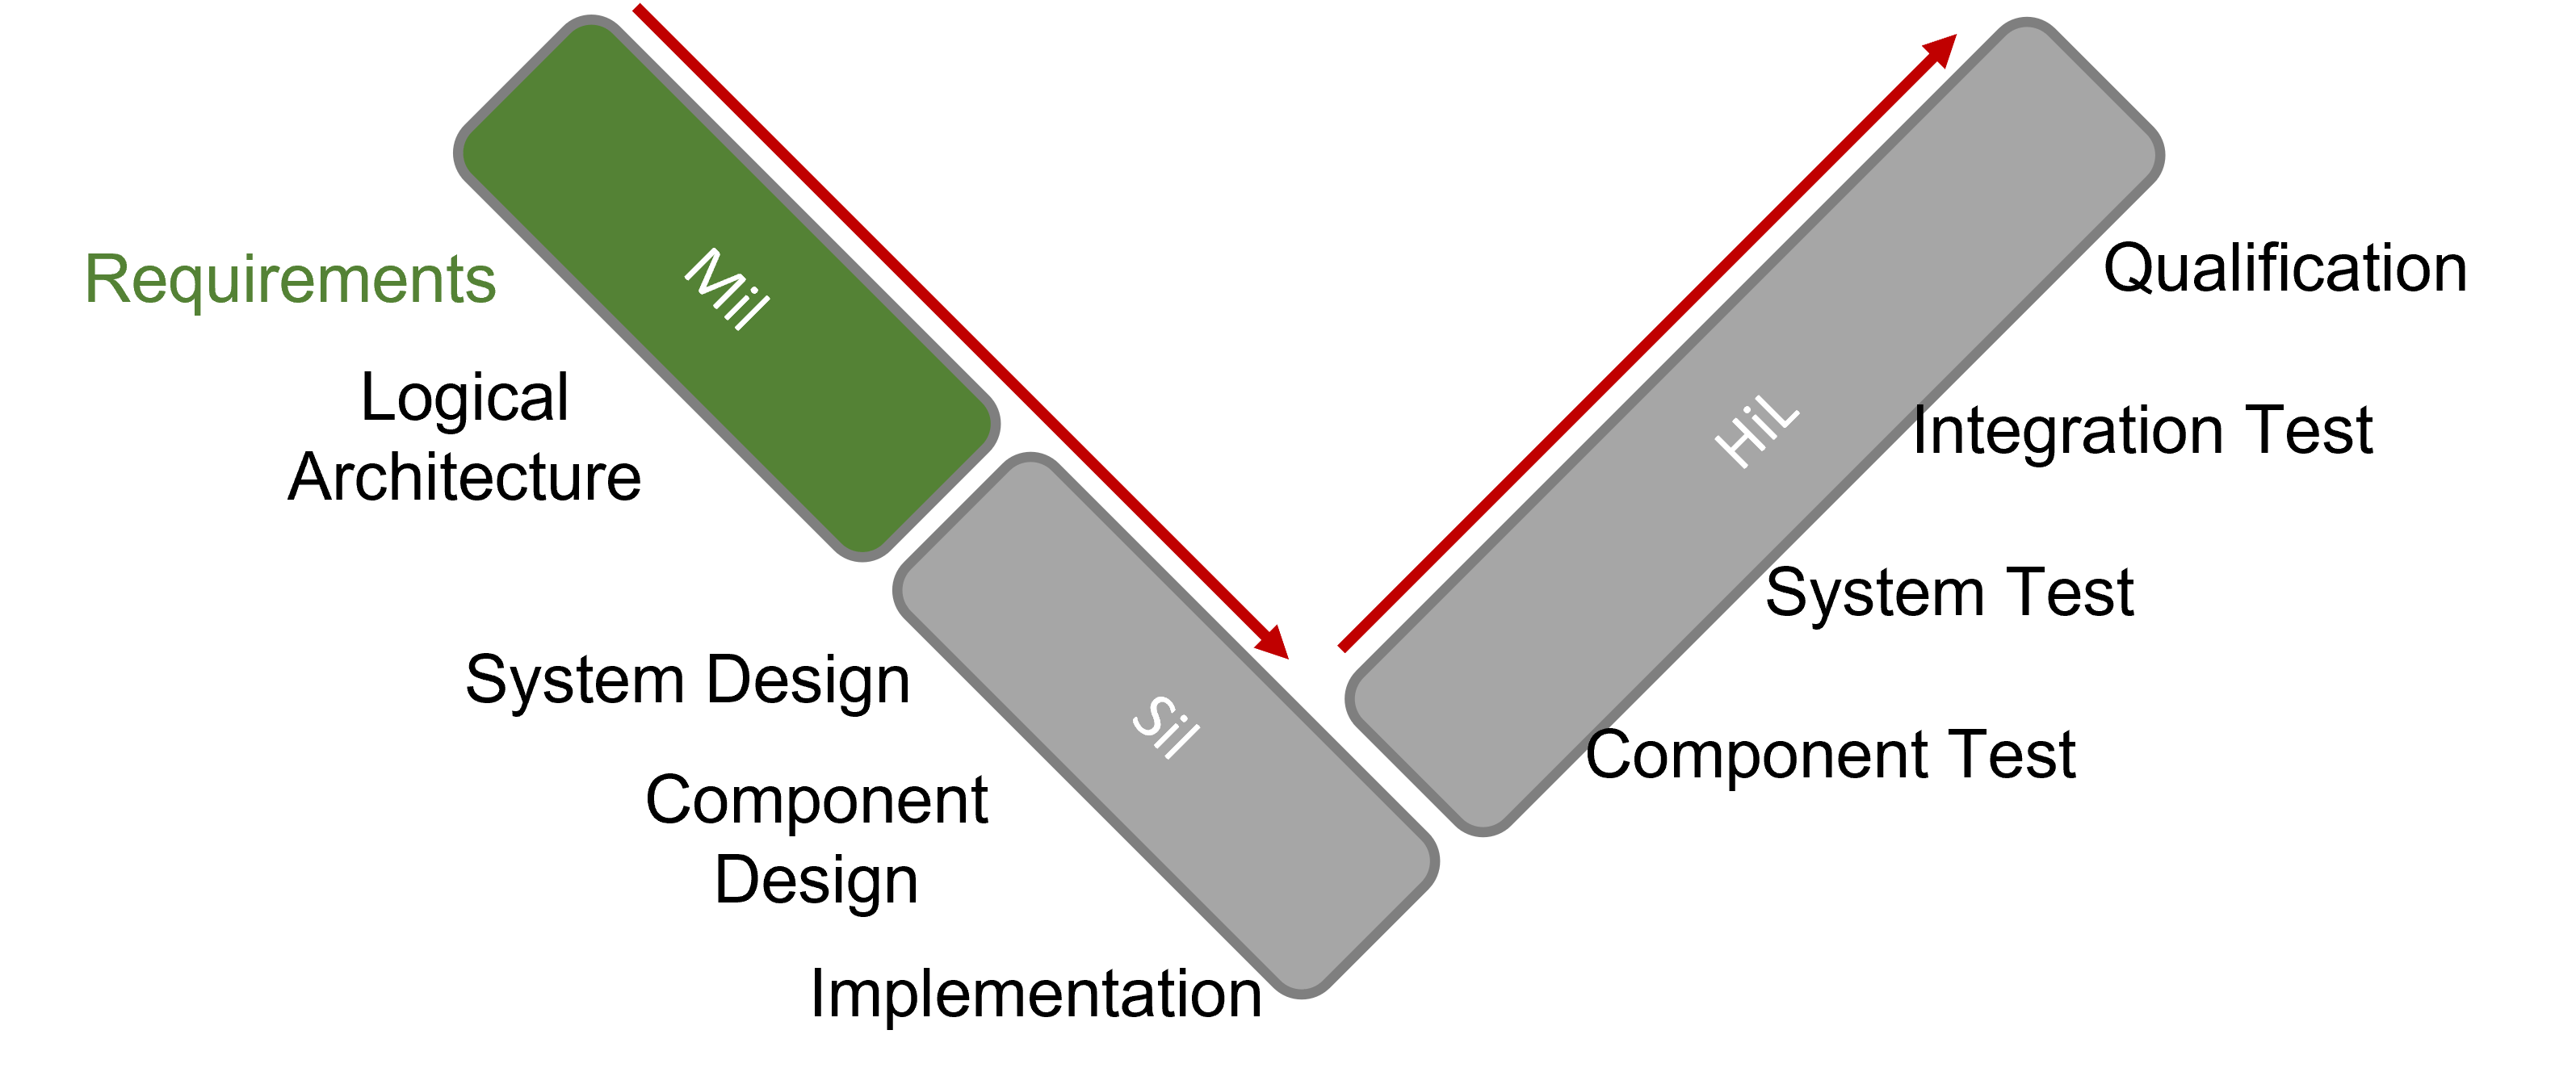
\includegraphics[width=12cm]{Pictures/V Model Requirements.png}
    \caption[V Model Requirements]{V Model Requirements Stage; Green - Developement status}
    \label{V Model Requirements}
    \end{center}
\end{figure}


\subsection{Requirements}
The developement of the System requirements was the first step in the developement process. This first step is one of the most important steps in the developement process, because it defines the functions and properties of all Systemcomponents.A selectoin of the requirements for the Human Machine Interface (HMI), the micro controller ($\mu$C), the motor and the motor controller are shown in Table \ref{Tab Key Requirements}. The full list of requirements can be found in Appendix \ref{AppendixRequirements}.

\begin{table}
    \centering
     \begin{tabular}{||c|c|c|c|c||} 
        \hline
        Req. Nr. & HMI & $\mu$C & Motor & Motor Controller \\ [0.5ex] 
        \hline\hline
        1 & Touch       & Real Time         &  Max. Torqe   & Closed Loop   \\ 
        2 & Modular     & Matlab Code Gen.  &  Min. Torqe   & Supply Voltage\\
        3 & UART Com.   & UART Com.         &  Max. Speed   & Programmable  \\
        4 & Separat PS  & Quad. Encoder     &  Min. Speed   & Resolution    \\
        5 & Mount       & GPIO              &  Space Claim  & Communication \\ [1ex] 
        \hline
     \end{tabular}
     \caption{Selection of Key Requirements for the ELS}
     \label{Tab Key Requirements}
\end{table}




\subsection{Logical Architecture}

The next step in the developement process of the ELS was to create the Logical Architecture of the System. This was done as a Toplevel Blockdiagramm as shown in Figure \ref{Logical Architecture}.

\begin{figure}
    \begin{center}
    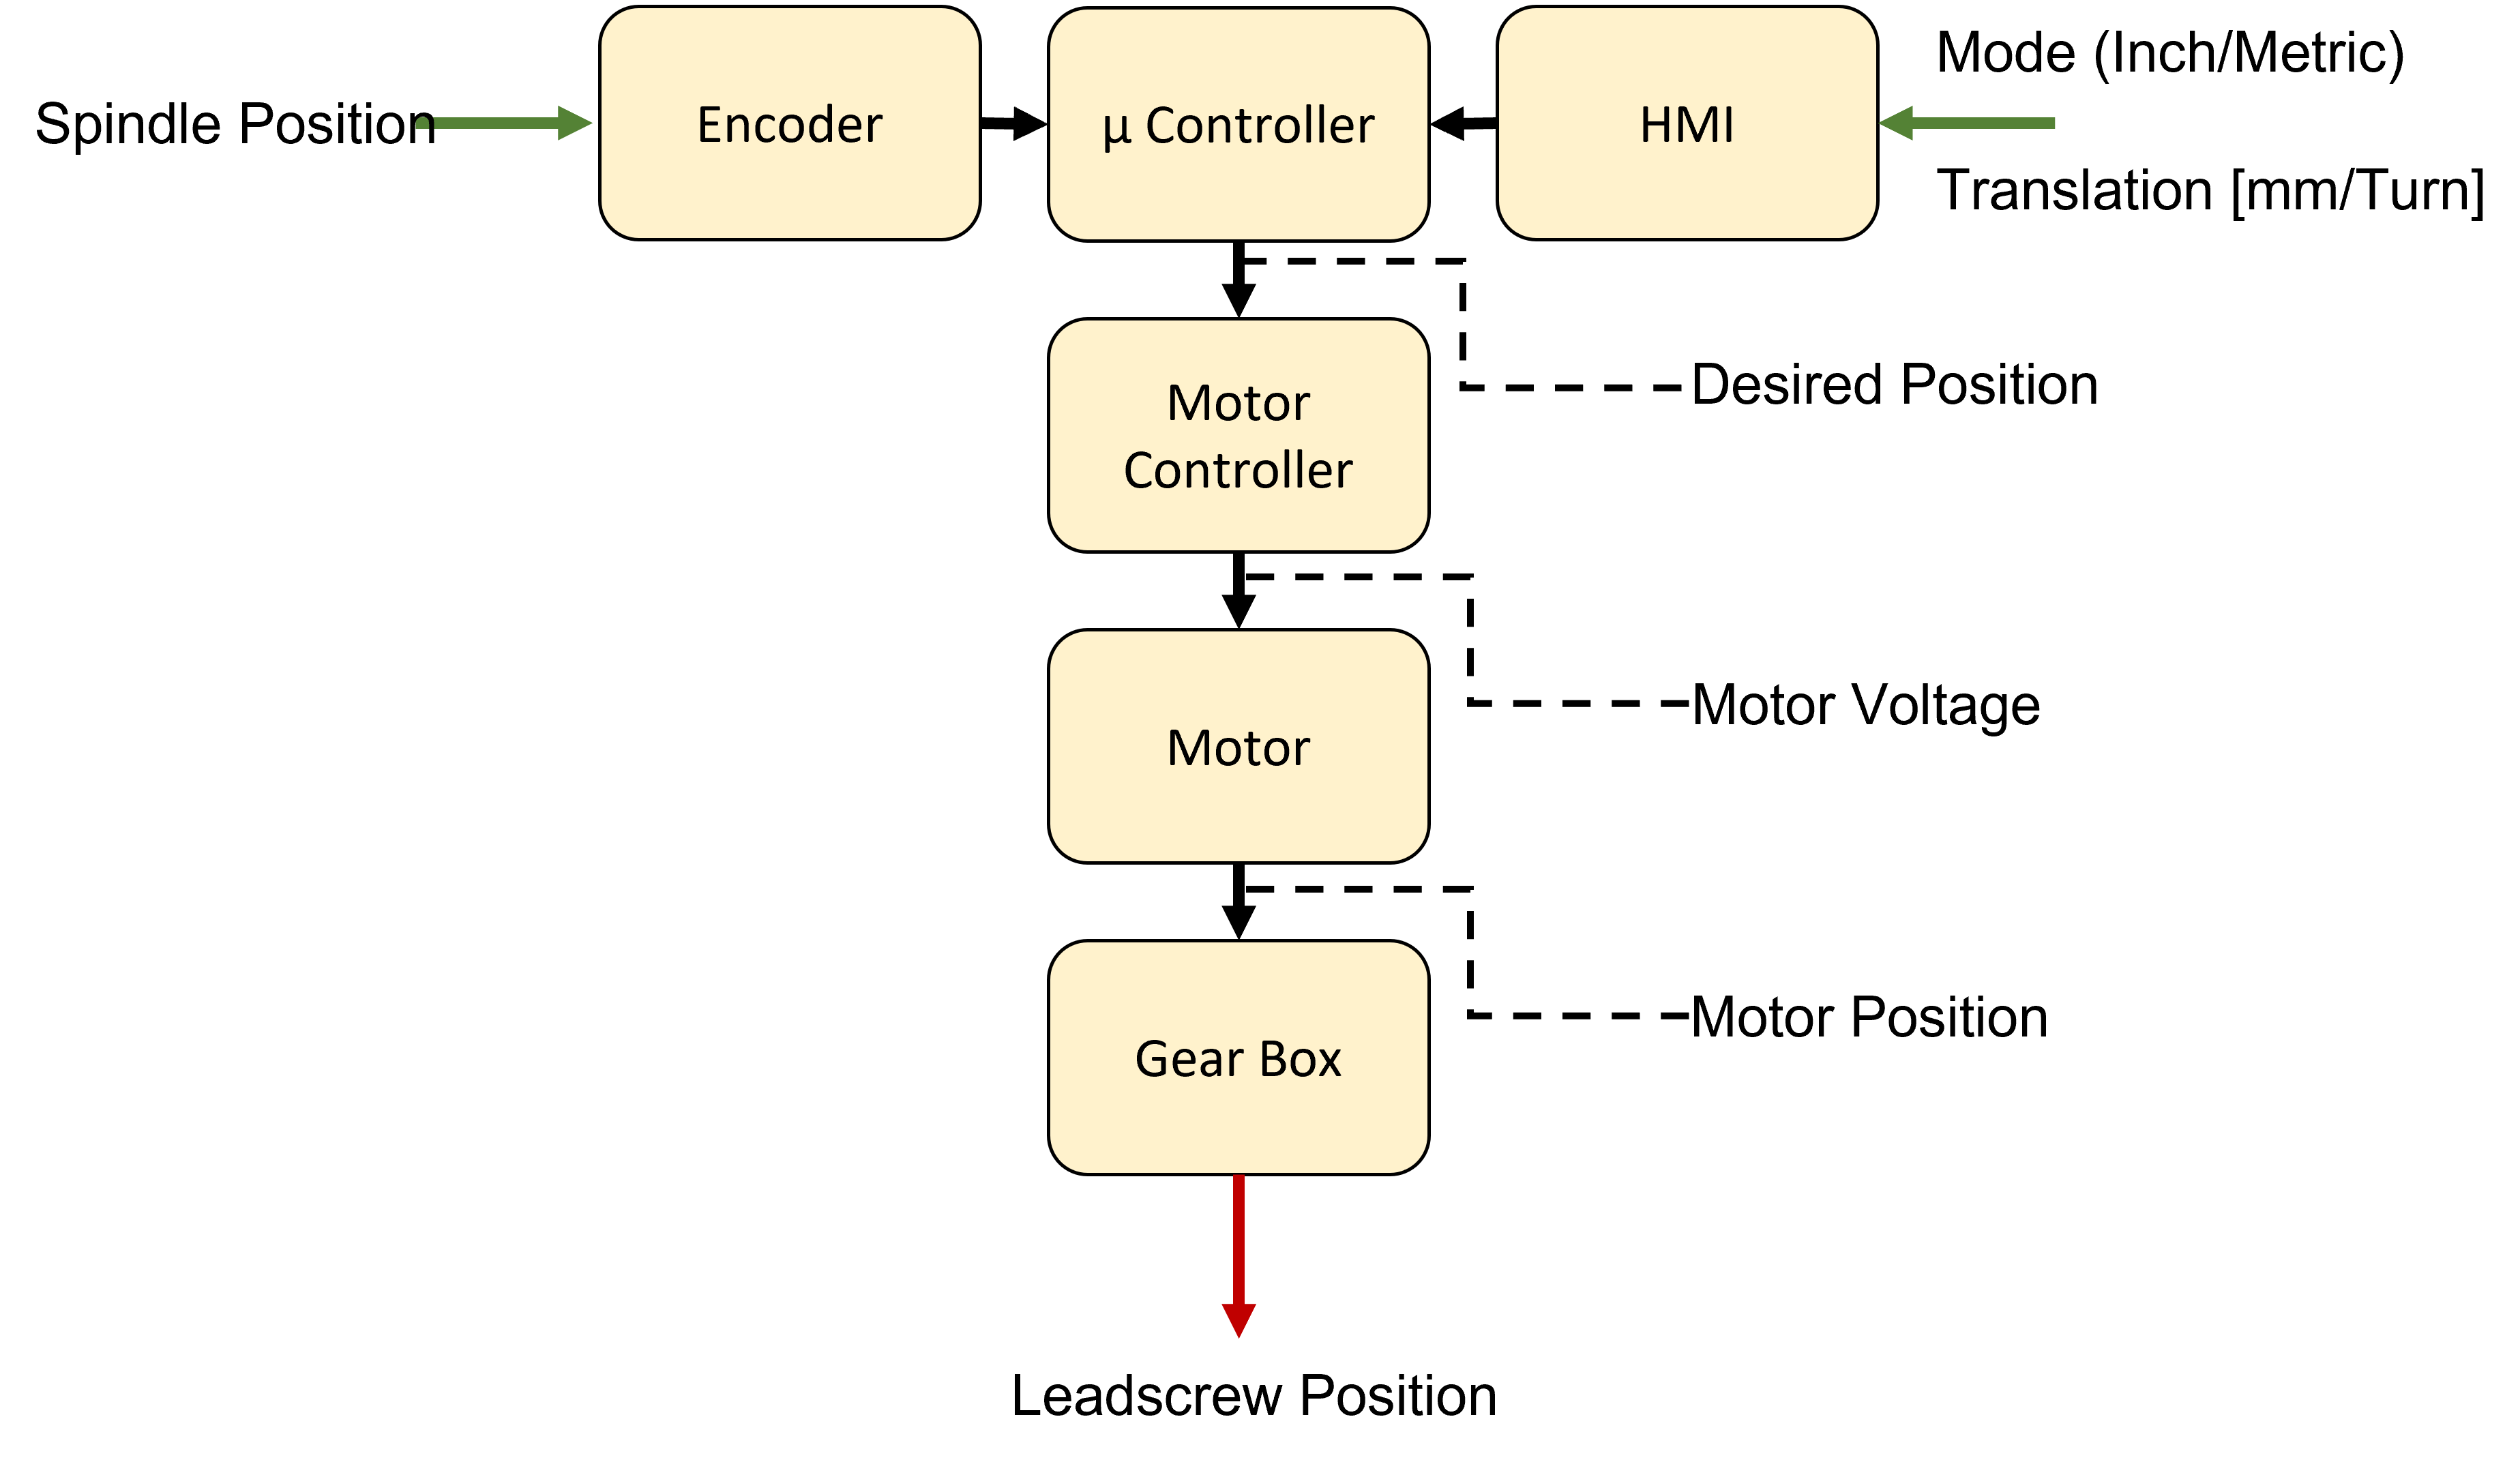
\includegraphics[width=12cm]{Pictures/Logical Architecture.png}
    \caption[Logical Architecture]{Logical Architecture}
    \label{Logical Architecture}
    \end{center}
\end{figure}

\section{System Design and Implementation}
This section describes the second half of the developement process, divided into system and component design as well as the integration of the components. This is the most time consuming process of the developement.For the system and component design, every function of each system and subsystem must be specified in detail. During the implementation phase, these functions are than transferred into the real system.\\
This developement stage is represented by the Software in the Loop (SIL) stage and is shown in Figure \ref{V Model System Design}.

\begin{figure}
    \begin{center}
    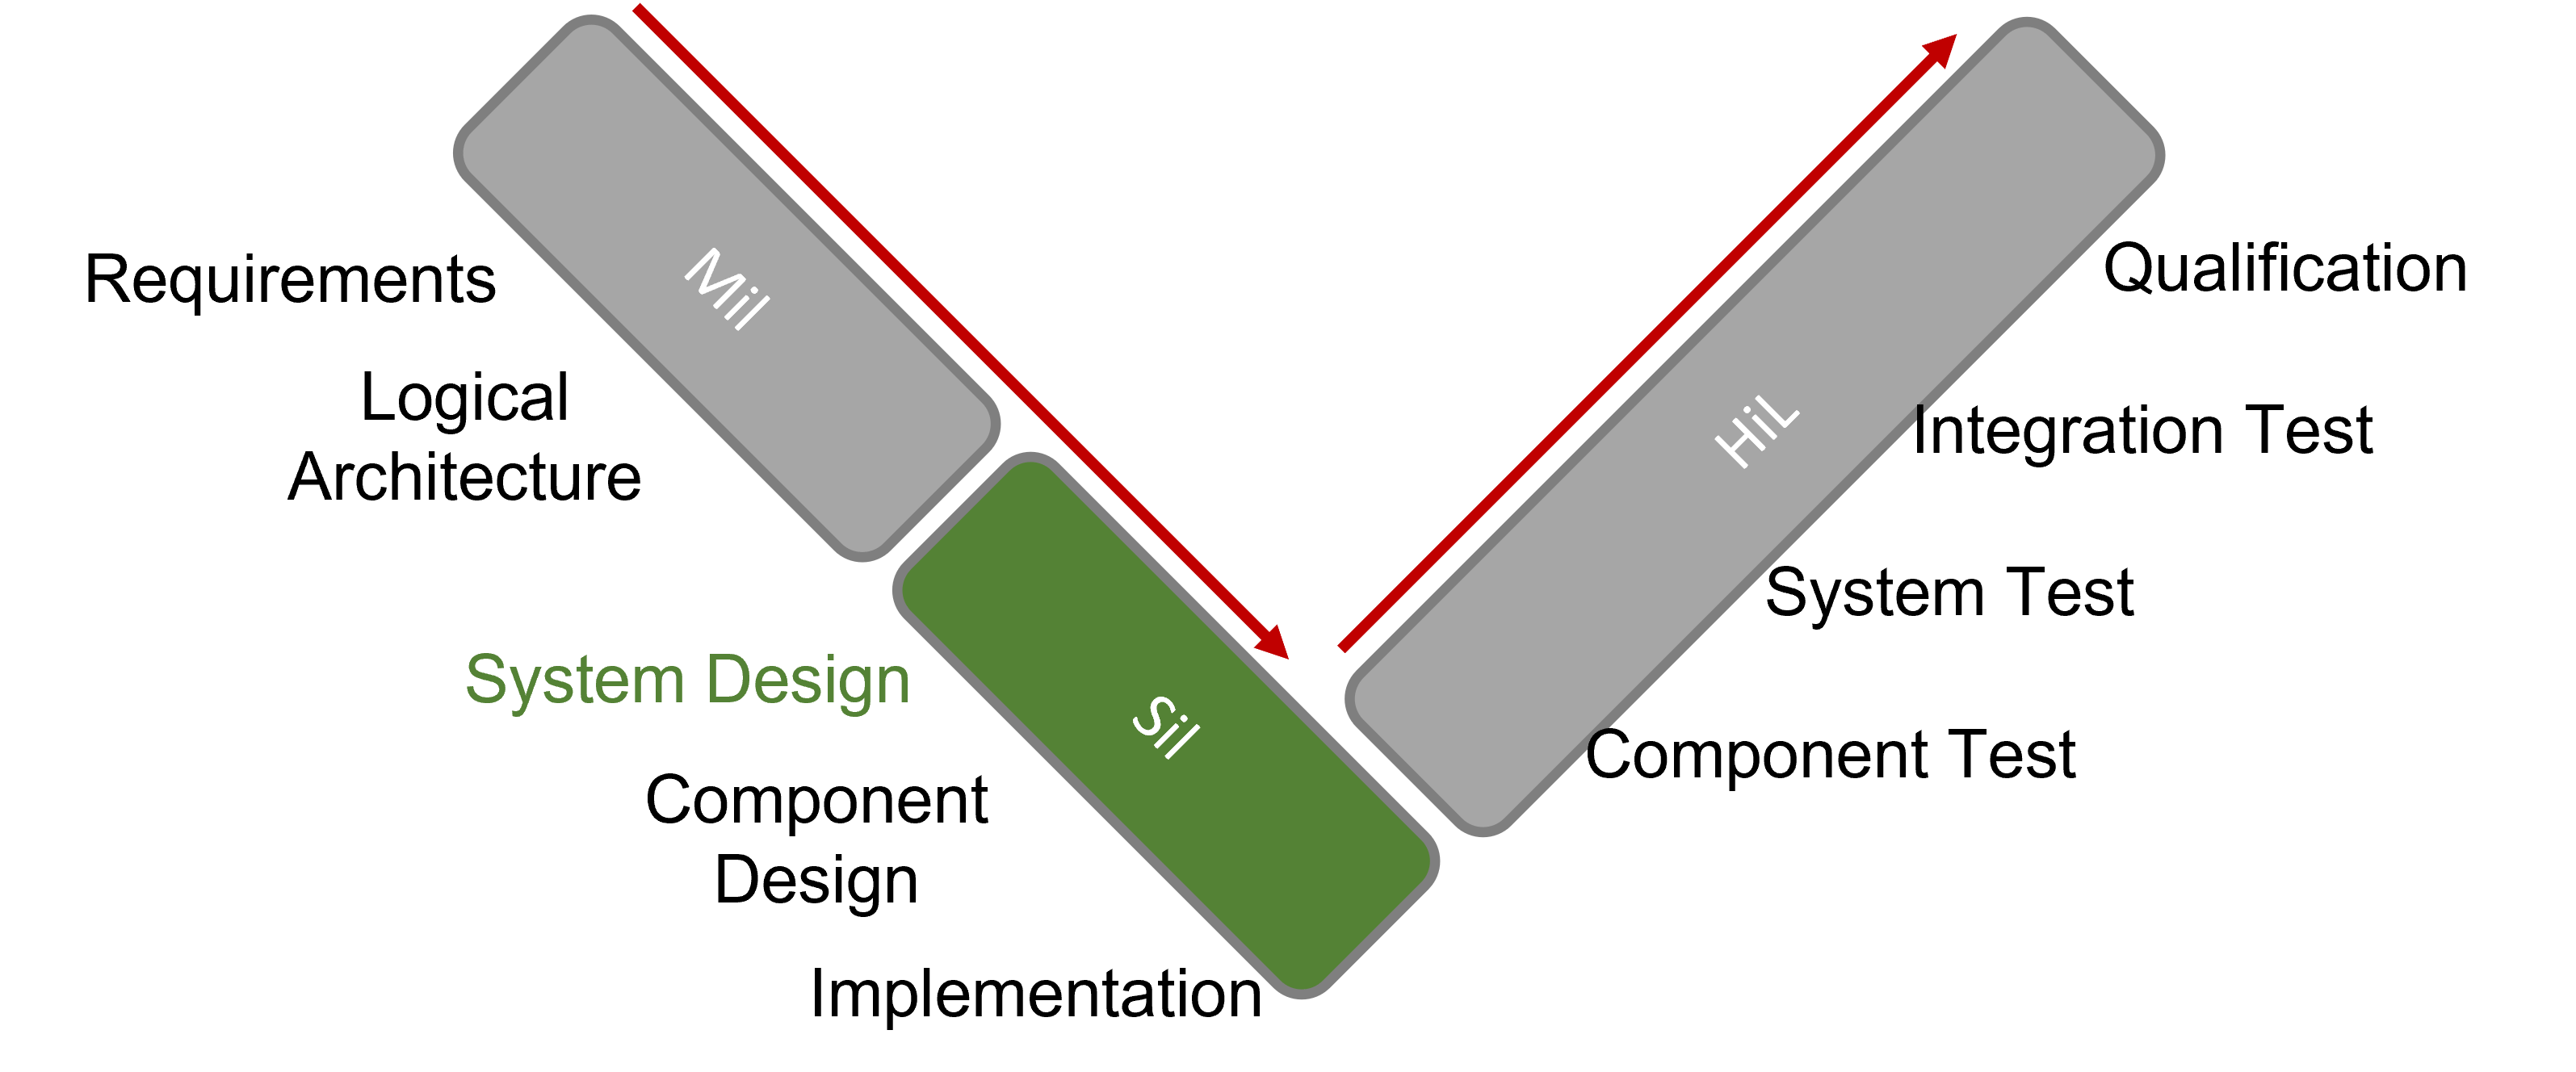
\includegraphics[width=12cm]{Pictures/V Model System Design.png}
    \caption[V Model System Design]{V Model SIL Stage; green - Developement steps SIL stage}
    \label{V Model System Design}
    \end{center}
\end{figure}

\subsection{System Design}
%%TODO: add Picture security pin
%%TODO: add Picture System design

The system design design is executed based on the previously developed system requirements and its logical architecture. The system design was approached by filling the requirements list as well as the block diagram of the logical architecture with component specific parameters. These parameters either need to be defined or found during the system design process.\\
A good example for this process is the required torque of the Leadscrew servo during a cutting process. This parameter can be found by measuring the power consumption of the AC motor for different cutting parameters with the old Leadscrew drive train. However while disassembling the original Leadscrew drive train in order to find a good place to mount the servo motor, an easier way to determine the required motor torque was found. In order to protect the Leadscrew the manufacturer secured the gear, that is driving the leadscrew with a brass pin. According to the manufacturer, this pin will shear off when more than 1.2Nm is acting on the leadscrew.\\
After this, all other parameter were determined in a similar matter. The resulting logical structure is shown in Figure \ref{System design}.

\begin{figure}
    \begin{center}
    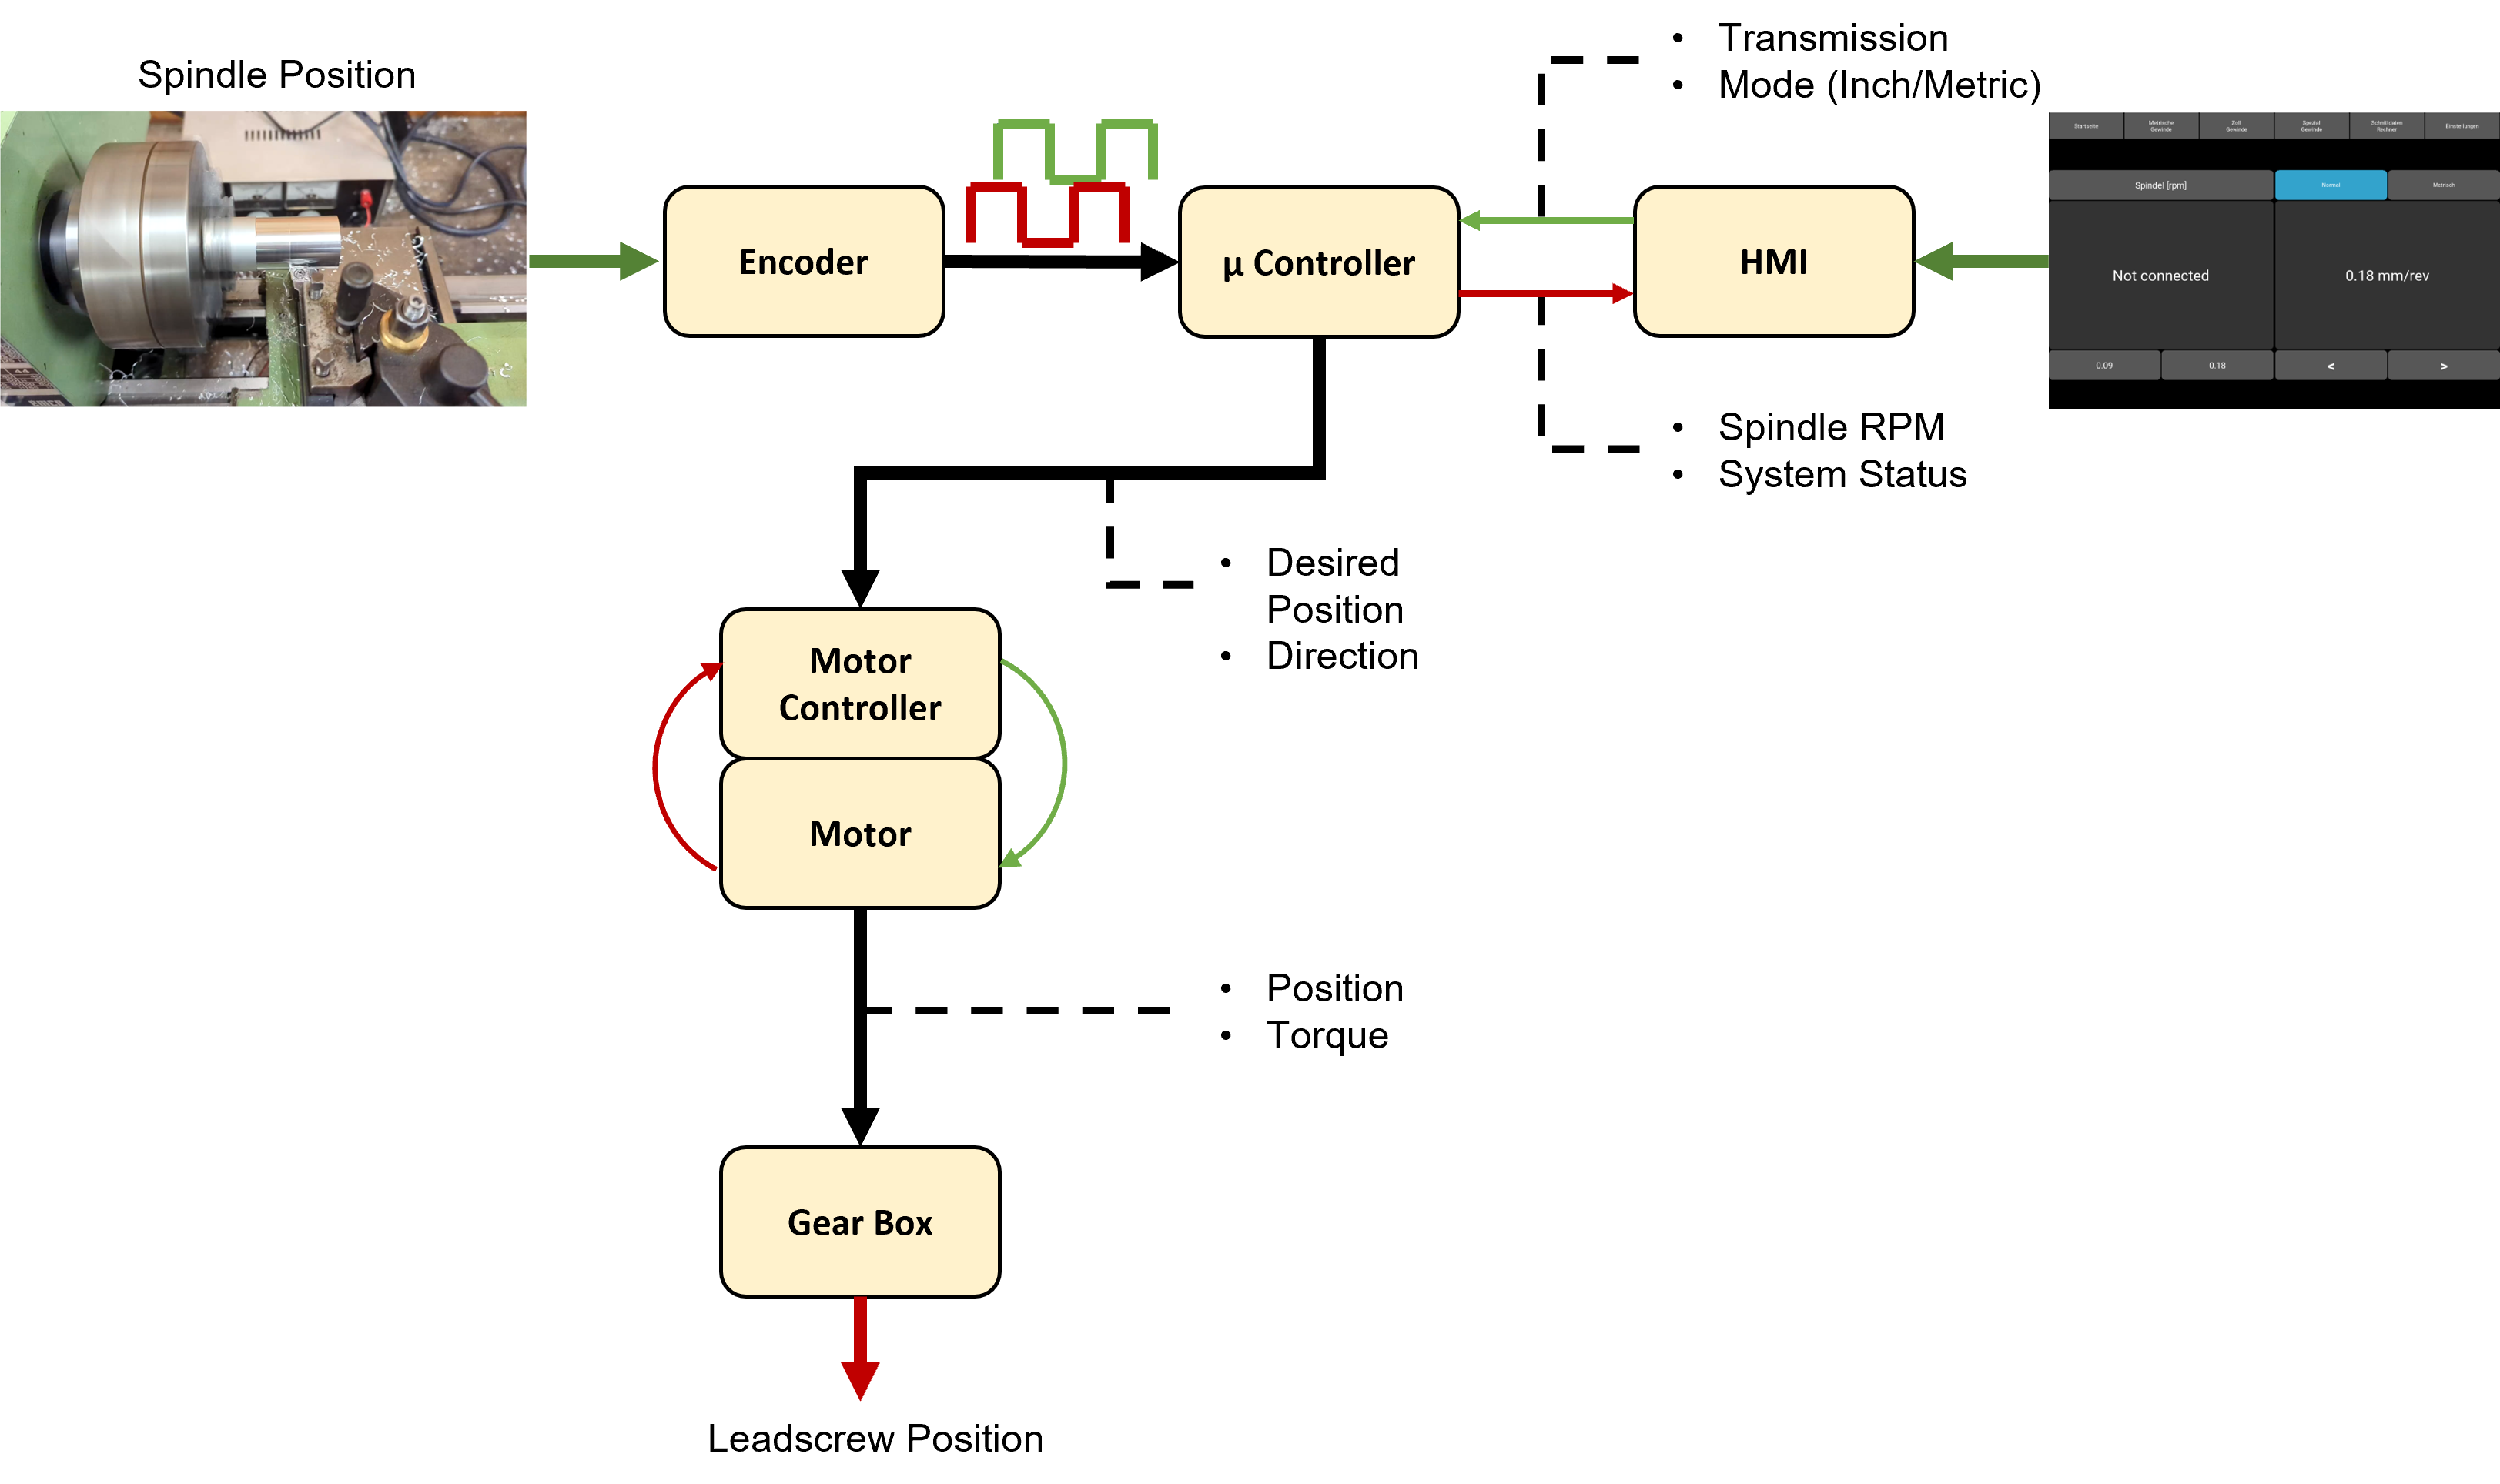
\includegraphics[width=12cm]{Pictures/SystemDesign.png}
    \caption[Block diagram of the system design]{Block diagram of the system design}
    \label{System design}
    \end{center}
\end{figure}


\subsection{Component Design}
During the component design phase, 
\subsubsection{HMI}
\subsubsection{Micro Controller}
\subsubsection{Encoder}
%%TODO Put Opkon in Appendix List of Companies
The design or in this case selection of the encoder was purely based on the previously defined requirements. The most significant requirements are shown in Table \ref{Tab Encoder Key Requirements}.

\begin{table}
    \centering
     \begin{tabular}{||c|c|c||} 
        \hline
        Req. Nr. & Requirement & Value\\ [0.5ex] 
        \hline\hline
        1 & Physical Size       & 60mm		\\ 
        2 & Supply Voltage      & 5V        \\
        3 & Resolution          & 4096 ppt  \\
        4 & Directional         & Yes       \\[1ex] 
        \hline
     \end{tabular}
     \caption{Selection of Key Requirements for the ELS}
     \label{Tab Encoder Key Requirements}
\end{table}

This lead to the selection of a Encoder from the manufacturer Opkon (see Appendix \ref{AppendixListOfCompanies}). The Encoder creates 4096 pulses/revolution, with half of them phase shifted by 90\degree in order to determine the turning direction. Further, the encoder covers an input voltage range from 5V - 30V, which is compatible with the Encoder Pins on the Launchpad XL. With a hight of 57mm, the Encoder just fits into the previously determined specifications.

\subsubsection{Motor and Motor Controller}
%%TODO Put Steppers Online in Appendix List of Companies
The motor was selected based the requirements list as well as recommendations from James Clough \cite{CloughELS}. The selected motor is from the company Steppers Online (see Appendix \ref{AppendixListOfCompanies}). It is a so called "integrated servo moter". This means, the motor consist of a brushless DC-motor, an encoder as well as the corresponding motor controller. All three of these parts are packaged into one unit as shown in Figure \ref{Integrated Servo Motor}.\\

\begin{figure}
    \begin{center}
    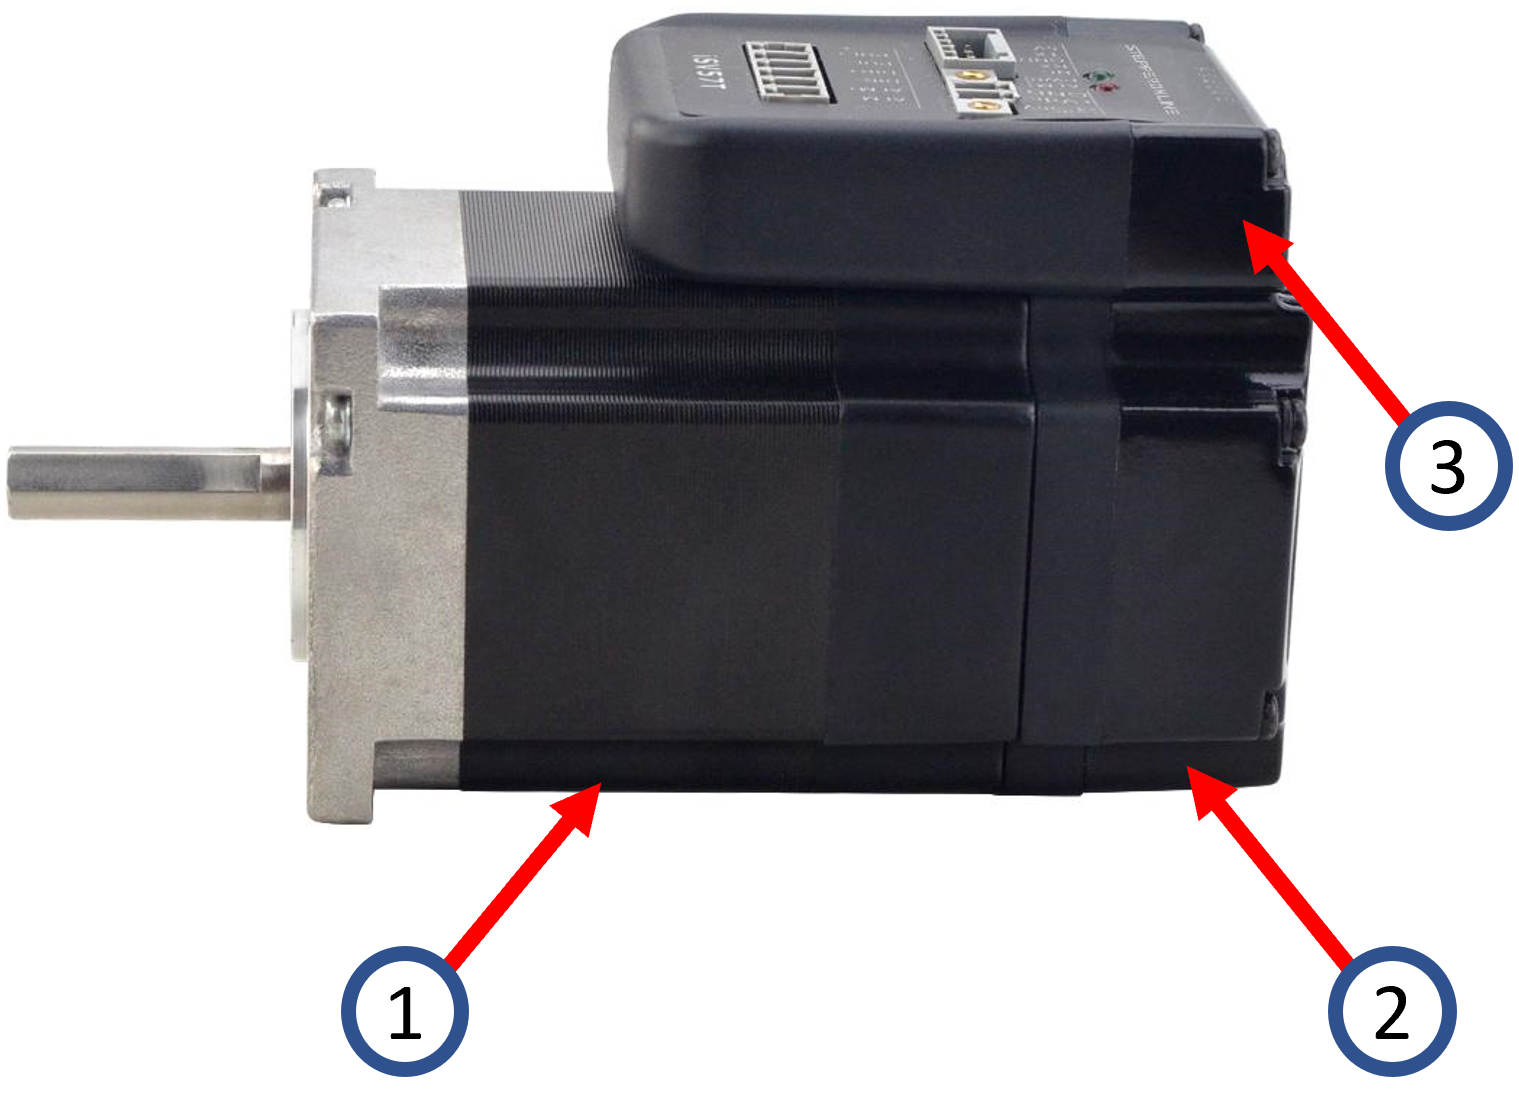
\includegraphics[width=12cm]{Pictures/IntegratedServo.png}
    \caption[Integrated Servo Motor]{Integrated Servo Motor; 1 - BLDC Motor, 2 - Encoder Unit, 3 - Control Unit}
    \label{Integrated Servo Motor}
    \end{center}
\end{figure}

The motor features an RPM range from 0 to 4000 rpm and a very constant maximum torque of 0.4 nm. Further, it has the right dimensions in order to fit the space claim requirements.\\
The motor controller in combination with the required software represent an easy programming interface. Via this interface, control parameters as well as parameter for the dynamics and precision of the motor can be set. As a starting value, the motor stiffness (responsiveness) gain was set to its maximum. Based on the software design of the micro controller, the precision of the motor was set to 2000 steps/revolution.\\
The interface to the motor is provided by a simple digital protocol. It consists of a direction and a step pin. The direction reacts to a logical 5V signal, where a logical 1 (5V) corresponds to clockwise rotation and a logical 0 (0V) corresponds to counterclockwise rotation. The step input reacts to logical pulses with a minimum pulse width of 1$\mu$s. Each puls will than move the motor by $\frac{1}{motor-resulution}$.

\subsubsection{Gearbox}
Because the motor is mounted underneath the Leadscrew, a a coupling between both elements was needed. This was done with the already existing gears from the old gearbox of the lathe. This decision was made because it needed the least modification (only a coupler from the motor to the gear had to be manufactured) and was the cheapest option. The gear ratio of 25/80 was selected to optimize the feed range of the lathe with the available RPM of the motor. This is shown in Figure \ref{Chart Leadscrew Dynamics}.

\begin{figure}
    \begin{center}
    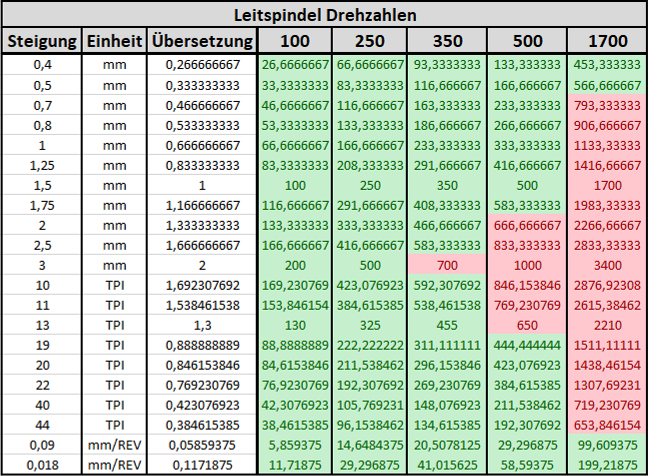
\includegraphics[width=12cm]{Pictures/TransmissionDynamics.png}
    \caption[Chart of the Leadscrew dynamics]{Chart of the Leadscrew dynamics; green - reachable Leadscrew RPM with a 25/80 transmission, red - not reachable Leadscrew RPM with a 25/80 transmission}
    \label{Chart Leadscrew Dynamics}
    \end{center}
\end{figure}

The transmission of the gearbox also increases the torque of the motor by a factor of 3.2. This way, the motor meets the specified torque of 1.2 Nm.



\section{System Testing}
\begin{figure}
    \begin{center}
    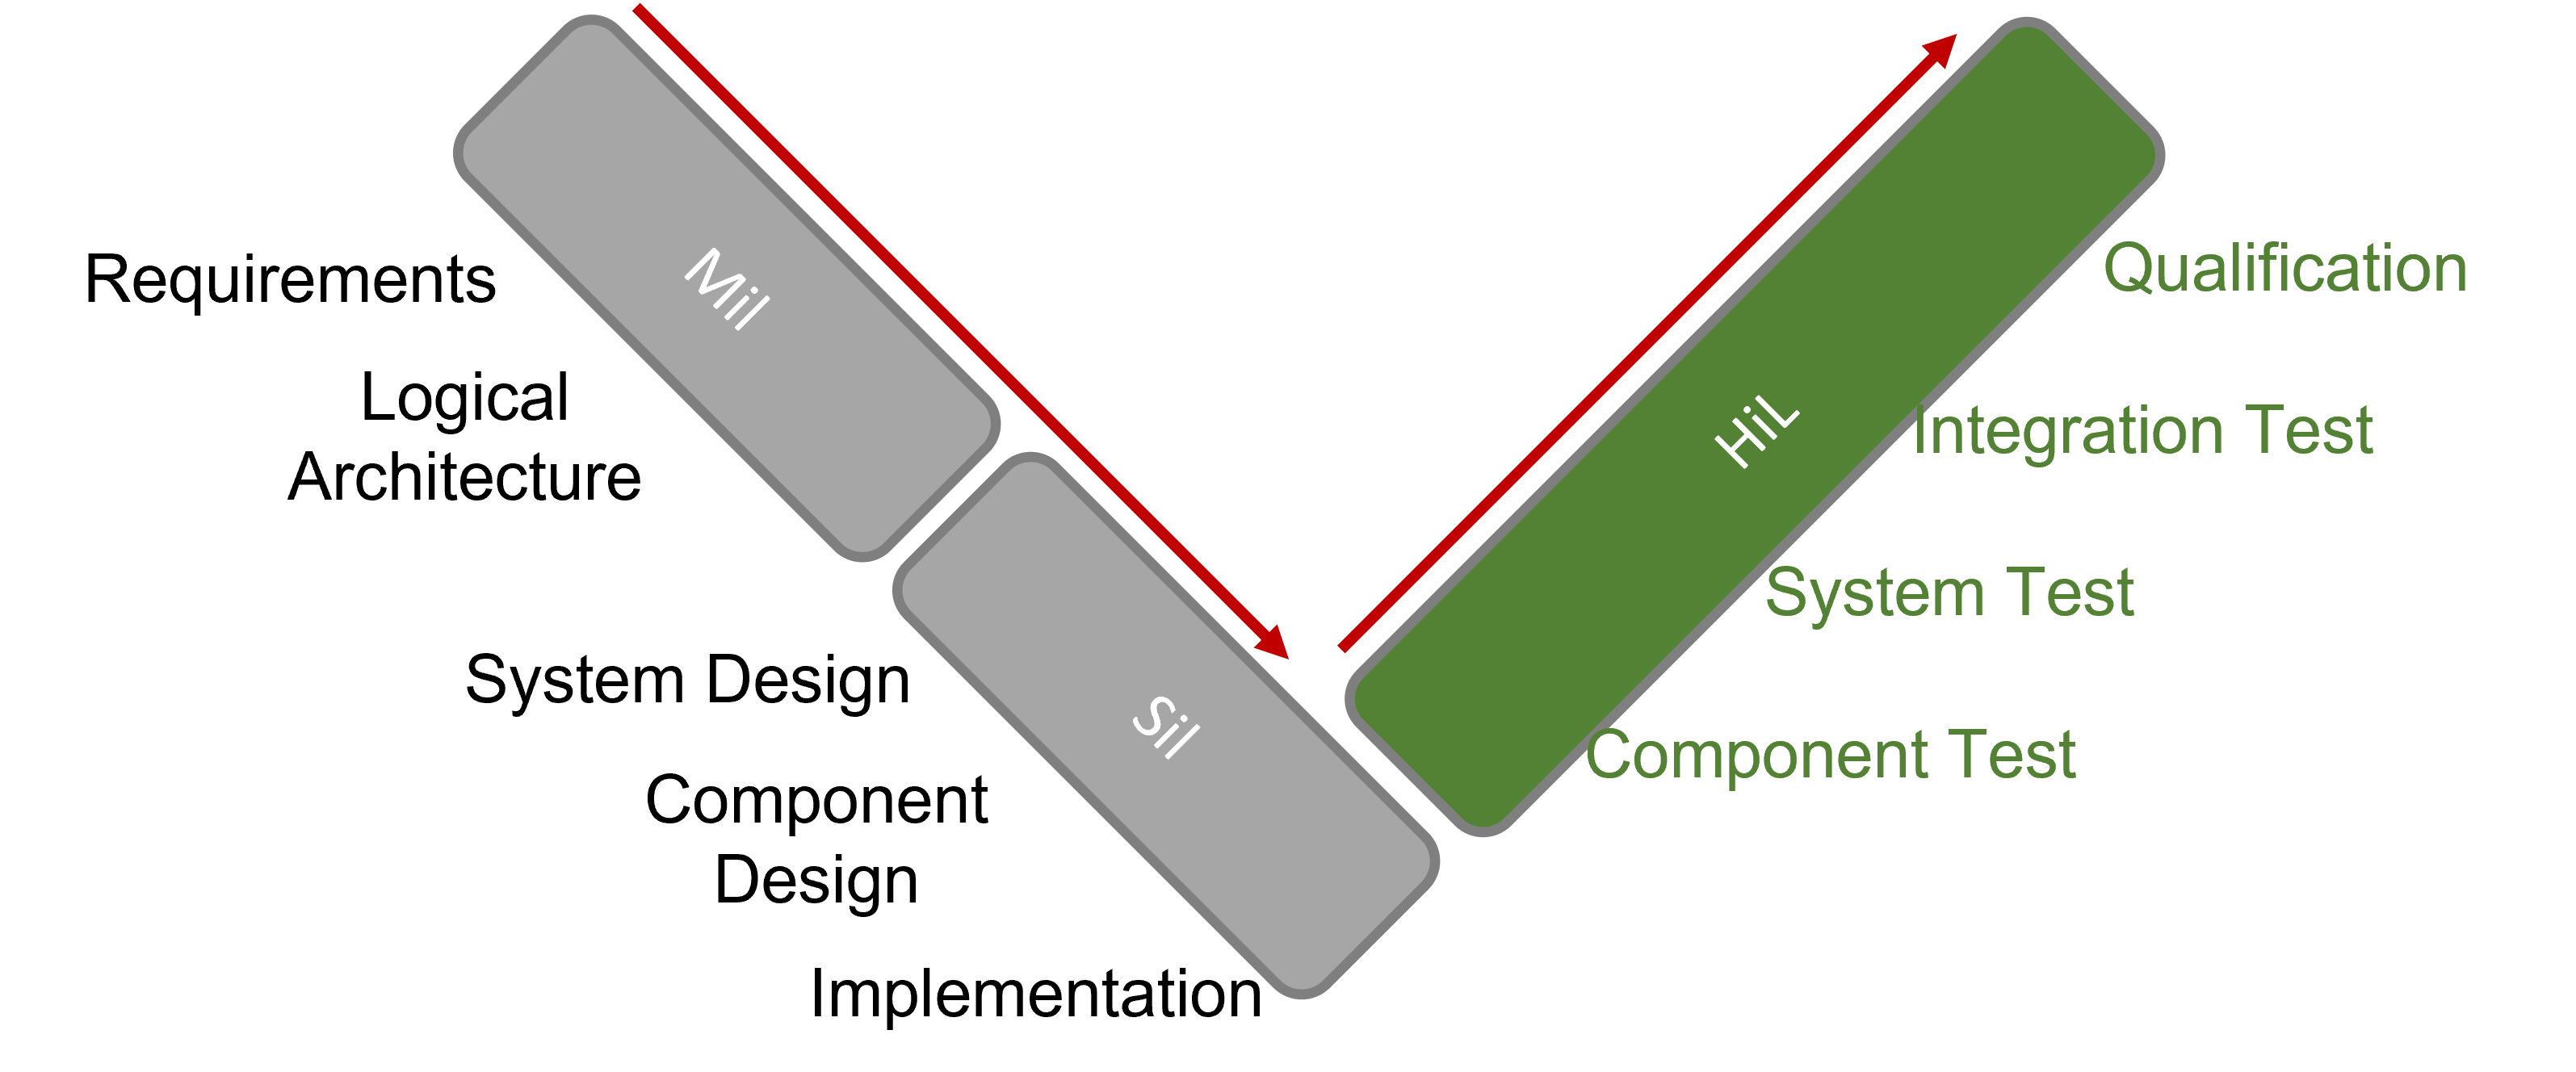
\includegraphics[width=12cm]{Pictures/V Model Component Test.png}
    \caption[V Model Component Test]{V Model Component Test Stage}
    \label{V Model Component Test}
    \end{center}
\end{figure}
\subsection{Component Test}
\subsubsection{Encoder}
\subsubsection{HMI}
\subsubsection{Micro Controller}
\subsubsection{Motor}
\subsubsection{Motor Controller}
\subsubsection{Gearbox}

\subsection{System Test}

\subsection{Integration Test}
\subsubsection{Turning}
\subsubsection{Threading}















\chapter{Results and Discussion}
\label{resultanddiscussion}
\section{Arithmetic}
\section{Turning}
\section{Threading}


\chapter{Outlook}
\label{outlook}



\listoffigures %Abbildungsverzeichnis

\listoftables %Tabellenverzeichnis

%\lstlistoflistings %Quelltextverzeichnis

%\printnomenclature %Abkürzungsverzeichnis

\renewcommand{\bibname}{References}
\printbibliography


%ANHANG
\cleardoublepage
\pagenumbering{Roman} %Big romanian Pagenumbering
\setcounter{page}{1} %Seitenzähler zurücksetzen

\thispagestyle{plain}
\appendix %Anhang einfügen


%TABLE OF CONTENTS APPENDIX
\phantomsection
\addcontentsline{toc}{chapter}{Appendix}
\startcontents[appendix]
\renewcommand\contentsname{\huge Appendix}% if a change of the default "Contents" name is required
\printcontents[appendix]{ }{0}{\section*{\contentsname}}
\stopcontents[main]
\newpage
%APPENDIX

\thispagestyle{empty}
\chapter{Additional Topics}
\label{AppendixAdditionalTopics}

% \begin{figure}[h!]
% \begin{center}
% \includegraphics[width=12cm]{Pictures/}
% \caption[}
% \label{OpticalTableCompliance}
% \end{center}
% \end{figure}


\thispagestyle{empty}
\chapter{List of Companies}
\label{AppendixListOfCompanies}

\begin{figure}[h!]

\includegraphics[height=1.6cm]{Pictures/EmcoLogo.png}
\end{figure}
\vspace{3mm}
Company:  EMCO GmbH\\
Website: \url{https://www.emco-world.com/}
\vspace{5mm}
\hrule
\vspace{10mm}

\begin{figure}[h!]

\includegraphics[height=1.6cm]{Pictures/KivyLogo.jpg}
\end{figure}
\vspace{3mm}
Company: Kivy.org\\
Website: \url{https://kivy.org/}
\vspace{5mm}
\hrule
\vspace{10mm}

\begin{figure}[h!]

\includegraphics[height=1.6cm]{Pictures/AppMathworksLogo}
\end{figure}
\vspace{3mm}
Company: The MathWorks, Inc.\\
Website: \url{https://www.mathworks.com/}
\vspace{5mm}
\hrule
\vspace{10mm}

\begin{figure}[h!]

\includegraphics[height=1.6cm]{Pictures/OpkonLogo.jpg}
\end{figure}
\vspace{3mm}
Company: OPKON Optic Electronic A.Ş.\\
Website: \url{https://www.opkon.com.tr/}
\vspace{5mm}
\hrule
\vspace{10mm}

\begin{figure}[h!]

\includegraphics[height=1.6cm]{Pictures/Raspberry_Pi_Logo.jpg}
\end{figure}
\vspace{3mm}
Company:  Raspberry Pi Foundation\\
Website: \url{https://www.raspberrypi.org/}
\vspace{5mm}
\hrule
\vspace{10mm}

\begin{figure}[h!]

\includegraphics[height=1.6cm]{Pictures/StepperonlineLogo.jpg}
\end{figure}
\vspace{3mm}
Company:  STEPPERONLINE, Inc.\\
Website: \url{https://www.omc-stepperonline.com/}
\vspace{5mm}
\hrule
\vspace{10mm}

\begin{figure}[h!]

\includegraphics[height=1.6cm]{Pictures/TexasInstruments-Logo.png}
\end{figure}
\vspace{3mm}
Company: Texas Instruments, Inc.\\
Website: \url{https://www.ti.com/}
\vspace{5mm}
\hrule
\vspace{10mm}



\thispagestyle{empty}
\chapter{Requirements ELS}
\label{AppendixRequirements}
\begin{figure}[!h]
    \begin{center}
    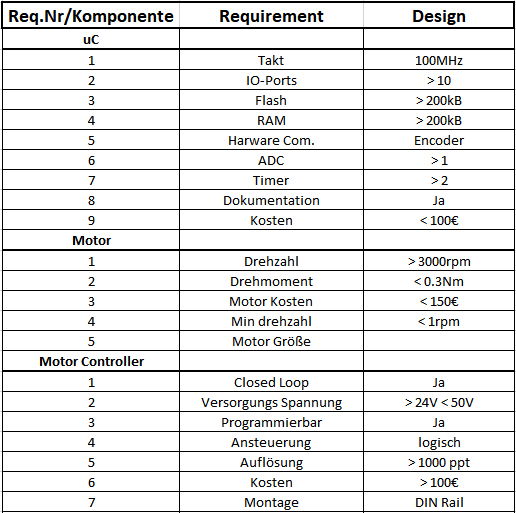
\includegraphics[width=12cm]{Pictures/AppRequ1.png}
    \caption[System requirements table 1]{System requirements table 1}
    \end{center}
\end{figure}

\begin{figure}[t]
    \begin{center}
    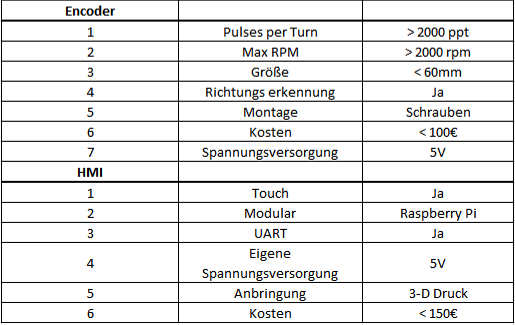
\includegraphics[width=12cm]{Pictures/AppRequ2.png}
    \caption[System requirements table 2]{System requirements table 2}
    \end{center}
\end{figure}

\thispagestyle{empty}
\chapter{Organisation Chart}
\label{AppChart}

\thispagestyle{empty}
\chapter{Source Code}
\label{appendixSoureCode}

\newpage
\section{C - Code}
\lstloadlanguages{Matlab}%
\lstinputlisting[language = Matlab, 
		firstline = 1, %Beginn bei Zeile XX aus Datei
		firstnumber = 1] %Beginn der Nummerierung 
		{./Sourcecode/TransmissionEvaluation.m} %{einzulesende Datei}
		

\newpage
\section{Python Code}
\lstloadlanguages{Matlab}%
\lstinputlisting[language = Matlab, 
		firstline = 1, %Beginn bei Zeile XX aus Datei
		firstnumber = 1] %Beginn der Nummerierung 
		{./Sourcecode/TransmissionEvaluation.m} %{einzulesende Datei}

\stopcontents[appendix]

%\begin{otherlanguage}{ngerman}
\addchap*{Eidesstattliche Erklärung}

\vspace*{5mm}

\thispagestyle{empty}

\begin{flushleft}
\begin{tabular}[h]{p{60mm}l p{60mm}l}
\textbf{Name:} Schwörer 			&\textbf{Vorname:} Lukas\\
\textbf{Matrikel-Nr.:} 65283		&\textbf{Studiengang:} Mechatronik\\
\end{tabular}
\end{flushleft}

\vspace*{11mm}

Hiermit versichere ich, \textbf{Lukas Schwörer}, an Eides statt, dass ich die vorliegende Bachelorarbeit

an der \textbf{University of Halmstad}

mit dem Titel \textbf{„Hard metrology of the human visual perception“}

selbständig und ohne fremde Hilfe verfasst und keine anderen als die angegebenen Hilfsmittel benutzt habe. Die Stellen der Arbeit, die dem Wortlaut oder dem Sinne nach anderen Werken entnommen wurden, sind in jedem Fall unter Angabe der Quelle kenntlich gemacht.\\

Ich habe die Bedeutung der eidesstattlichen Versicherung und prüfungsrechtlichen Folgen (\S 23 Abs. 3 des allg. Teils der Bachelor-SPO der Hochschule Aalen) sowie die strafrechtlichen Folgen (siehe unten) einer unrichtigen oder unvollständigen eidesstattlichen Versicherung zur Kenntnis genommen.\\

\vspace*{10mm}
\Large\textbf{Auszug aus dem Strafgesetzbuch (StGB)}


\normalsize\textbf{\S 156 StGB} Falsche Versicherung an Eides Statt
Wer von einer zur Abnahme einer Versicherung an Eides Statt zuständigen Behörde eine solche Versicherung falsch abgibt oder unter Berufung auf eine solche Versicherung falsch aussagt, wird mit Freiheitsstrafe bis zu drei Jahren oder mit Geldstrafe bestraft.

\vspace*{25mm}


\rule[-0.2cm]{5cm}{0.5pt} \hspace*{30mm}\rule[-0.2cm]{5cm}{0.5pt}
\newline
Ort, Datum\hspace*{61.85mm}Unterschrift

\end{otherlanguage} 


\end{document}
%%%%%%%%%%%%%%%%%%%%%%%%%%%%%%%%%%%%%%%%%%%%%%%%%%%%%%%%%%%%
%END_OF_FILE















